\documentclass[lang=cn]{elegantpaper}

\title{十一月过程性研究记录}
\author{陶理}
\usepackage{listings}
\begin{document}
\date{November 28, 2023}
\maketitle

\begin{abstract}
    该份过程性研究记录(截止至撰写日期)主要记录了作者在十一月所完成的研究成果。主要有以下几项:
    \begin{enumerate}
        \item 对普通话的语音指令数据进行处理:如声谱图等特征
        \item 对处理后的数据进行分析
    \end{enumerate}
\end{abstract}

\section{普通话语音指令数据的处理和特征提取}
\subsection{数据收集}
出于方便考虑,我打算先采集普通话语音指令的数据进行分析再将一些结论推广到方言上进行调整。另外,由于普通话和方言都属于汉语,所以发语逻辑基本相同,因此采集普通话也是有其合理性的。
由于时间紧张,先采集了22条基本的语音指令进行分析。数据随本份过程性研究记录一齐上传。
\subsection{声谱图}
\textbf{定义}:声谱图(voicegram)又称时频谱(英语:Spectrogram),是一种描述波动的各频率成分如何随时间变化的热图。
利用傅里叶变换得到的传统的2维频谱可展示复杂的波动是如何按比例分解为简单波的叠加(分解为频谱),但是无法同时体现它们随时间的变化。
能对波动的时间变量与频率分布同时进行分析的常用数学方法是短时距傅里叶变换,但是直接绘成3维图像的话又不便于在纸面上观察和分析。时频谱在借助时频分析方法的基础上,以热图的形式将第3维的数值用颜色的深浅加以呈现。\textit{源自维基百科}

以下是一个使用Python语言生成声谱图的示例:
\begin{figure}[h]
    \centering
    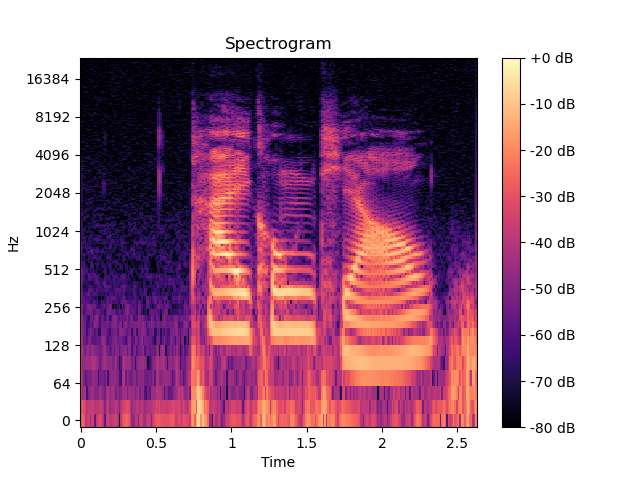
\includegraphics[width=0.5\textwidth]{testspectrogram.png}
\end{figure}
\begin{lstlisting}[language=Python]
import librosa
import librosa.display
import matplotlib.pyplot as plt
import numpy as np
audio_path = ''
y, sr = librosa.load(audio_path, sr=None)
D = np.abs(librosa.stft(y))
spec = librosa.amplitude_to_db(D, ref=np.max)
energy_per_frame = np.sum(D**2, axis=0)
librosa.display.specshow(spec, y_axis='log', x_axis='time', sr=sr)
plt.colorbar(format='%+2.0f dB')
plt.title('Spectrogram')
plt.show()
\end{lstlisting}
接下来,我对目前所有22条数据进行声谱图的绘制,结果如下:
\begin{figure}[h]
    \centering
    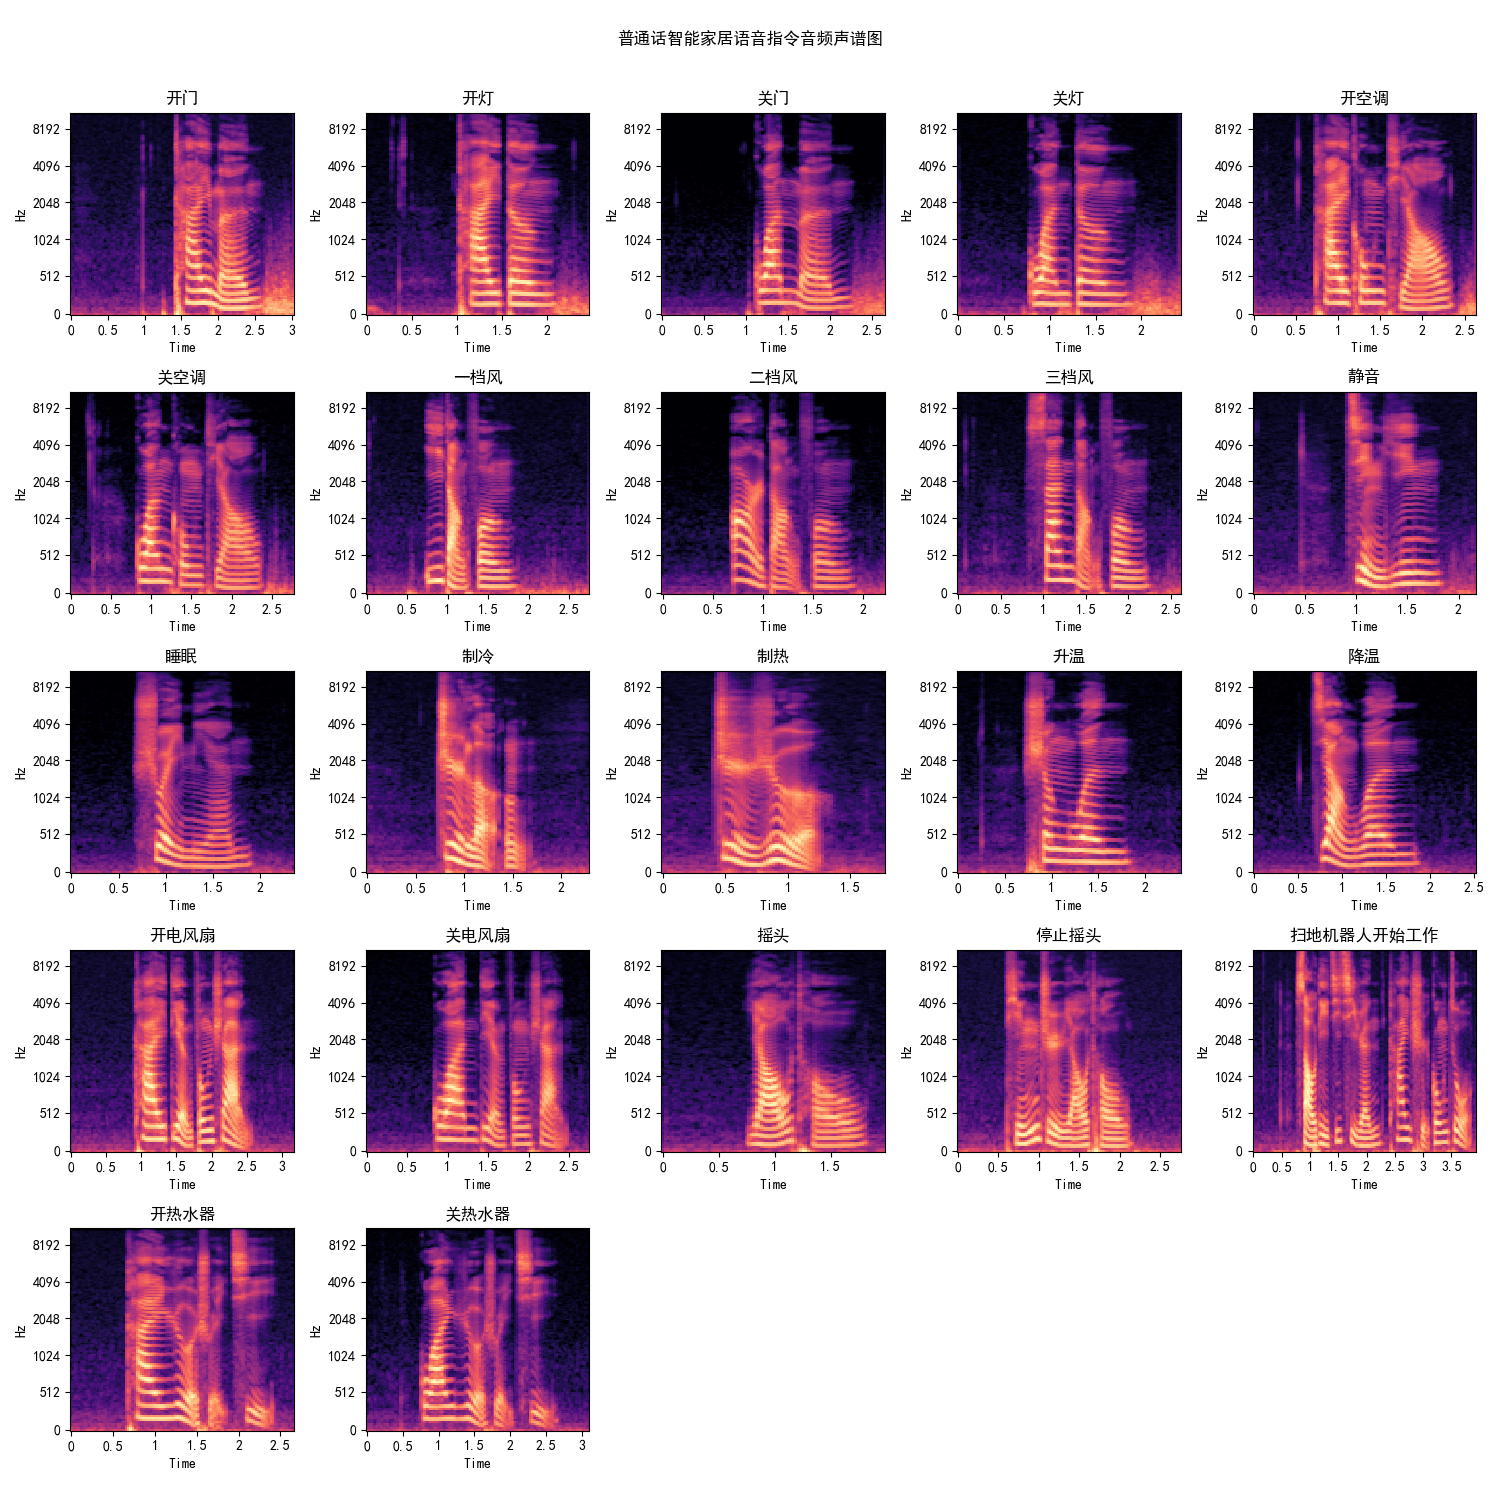
\includegraphics[width=0.9\textwidth]{spectrogram.png}
\end{figure}
程序如下:
\begin{lstlisting}[language=Python]
import librosa
import librosa.display
import matplotlib.pyplot as plt
import numpy as np
plt.rcParams['font.sans-serif'] = ['SimHei']
def generate_spectrogram(audio_file):
    y, sr = librosa.load(audio_file)
    spectrogram = librosa.feature.melspectrogram(y=y, sr=sr)
    return librosa.power_to_db(spectrogram, ref=np.max), sr
spectrograms = []
srs = []
for i in range(1, 23):
    audio_file = '...'
    spectrogram, sr = generate_spectrogram(audio_file)
    spectrograms.append(spectrogram)
    srs.append(sr)
fig, axes = plt.subplots(nrows=5, ncols=5, figsize=(15, 15))
title = ['...','...',...,'...','...']
for i in range(22):
    row = i // 5
    col = i % 5
    ax = axes[row, col]
    librosa.display.specshow(spectrograms[i], sr=srs[i], x_axis='time', y_axis='mel', ax=ax)
    ax.set_title(title[i])
num_images = 22
num_rows = 5
num_cols = 5
for i in range(num_images, num_rows * num_cols):
    fig.delaxes(axes.flatten()[i])
plt.tight_layout(rect=[0, 0.01, 1, 0.95])
plt.suptitle('...')
plt.savefig('...')
plt.show()
\end{lstlisting}
\end{document}